%%%%%%%%%%%%%%%%%%%%%%%%%%%%%%%%%%%%%%%%%
% Beamer Presentation
% LaTeX Template
% Version 1.0 (10/11/12)
%
% This template has been downloaded from:
% http://www.LaTeXTemplates.com
%
% License:
% CC BY-NC-SA 3.0 (http://creativecommons.org/licenses/by-nc-sa/3.0/)
%
%%%%%%%%%%%%%%%%%%%%%%%%%%%%%%%%%%%%%%%%%

%----------------------------------------------------------------------------------------
%	PACKAGES AND THEMES
%----------------------------------------------------------------------------------------

\documentclass{beamer}

\mode<presentation> {

% The Beamer class comes with a number of default slide themes
% which change the colors and layouts of slides. Below this is a list
% of all the themes, uncomment each in turn to see what they look like.

%\usetheme{default}
%\usetheme{AnnArbor}
%\usetheme{Antibes}
%\usetheme{Bergen}
%\usetheme{Berkeley}
%\usetheme{Berlin}
%\usetheme{Boadilla}
%\usetheme{CambridgeUS}
%\usetheme{Copenhagen}
%\usetheme{Darmstadt}
%\usetheme{Dresden}
%\usetheme{Frankfurt}
%\usetheme{Goettingen}
%\usetheme{Hannover}
%\usetheme{Ilmenau}
%\usetheme{JuanLesPins}
%\usetheme{Luebeck}
\usetheme{Madrid}
%\usetheme{Malmoe}
%\usetheme{Marburg}
%\usetheme{Montpellier}
%\usetheme{PaloAlto}
%\usetheme{Pittsburgh}
%\usetheme{Rochester}
%\usetheme{Singapore}
%\usetheme{Szeged}
%\usetheme{Warsaw}

% As well as themes, the Beamer class has a number of color themes
% for any slide theme. Uncomment each of these in turn to see how it
% changes the colors of your current slide theme.

%\usecolortheme{albatross}
%\usecolortheme{beaver}
%\usecolortheme{beetle}
%\usecolortheme{crane}
%\usecolortheme{dolphin}
%\usecolortheme{dove}
%\usecolortheme{fly}
%\usecolortheme{lily}
%\usecolortheme{orchid}
%\usecolortheme{rose}
%\usecolortheme{seagull}
%\usecolortheme{seahorse}
%\usecolortheme{whale}
%\usecolortheme{wolverine}

%\setbeamertemplate{footline} % To remove the footer line in all slides uncomment this line
%\setbeamertemplate{footline}[page number] % To replace the footer line in all slides with a simple slide count uncomment this line

%\setbeamertemplate{navigation symbols}{} % To remove the navigation symbols from the bottom of all slides uncomment this line
}

\usepackage{graphicx} % Allows including images
\usepackage{booktabs} % Allows the use of \toprule, \midrule and \bottomrule in tables

%----------------------------------------------------------------------------------------
%	TITLE PAGE
%----------------------------------------------------------------------------------------

\title[RTABMap / \textit{Guidance} SLAM]{Map Building via \textit{RTABMap} and \textit{Guidance}} % The short title appears at the bottom of every slide, the full title is only on the title page

\author{Steve McGuire} % Your name
\institute[] % Your institution as it will appear on the bottom of every slide, may be shorthand to save space
{
University of Colorado at Boulder \\ % Your institution for the title page
\medskip
\textit{} % Your email address
}
\date{October 14th, 2015} % Date, can be changed to a custom date

\begin{document}

\begin{frame}
\titlepage % Print the title page as the first slide
\end{frame}

\begin{frame}
\frametitle{Overview} % Table of contents slide, comment this block out to remove it
\tableofcontents % Throughout your presentation, if you choose to use \section{} and \subsection{} commands, these will automatically be printed on this slide as an overview of your presentation
\end{frame}

%----------------------------------------------------------------------------------------
%	PRESENTATION SLIDES
%----------------------------------------------------------------------------------------

%------------------------------------------------
\section{Problem Statement} % Sections can be created in order to organize your presentation into discrete blocks, all sections and subsections are automatically printed in the table of contents as an overview of the talk
%------------------------------------------------
\begin{frame}
\frametitle{Problem Statement}
\textbf{Statement:}
Given a set of sensors, produce a metrically accurate 3-D map of the world while estimating observation location and motion in that map.

%\begin{figure}
%\includegraphics[width=0.9\linewidth]{figures/Problem_Setup}
%\caption{\textbf{Coordinate System Diagram}}
%\end{figure}
\end{frame}

\section{Sensor Details}

\begin{frame}
\frametitle{Sensor Suite}
\begin{itemize}
\item{\textit{Inertial}} 6DOF inertial data is available with calibration parameters
\item{\textit{Depth}} Dense metric depth imagery is available with a pinhole camera model
\item{\textit{Visual}} Imagery is available with a pinhole camera model
\end{itemize}
\begin{figure}
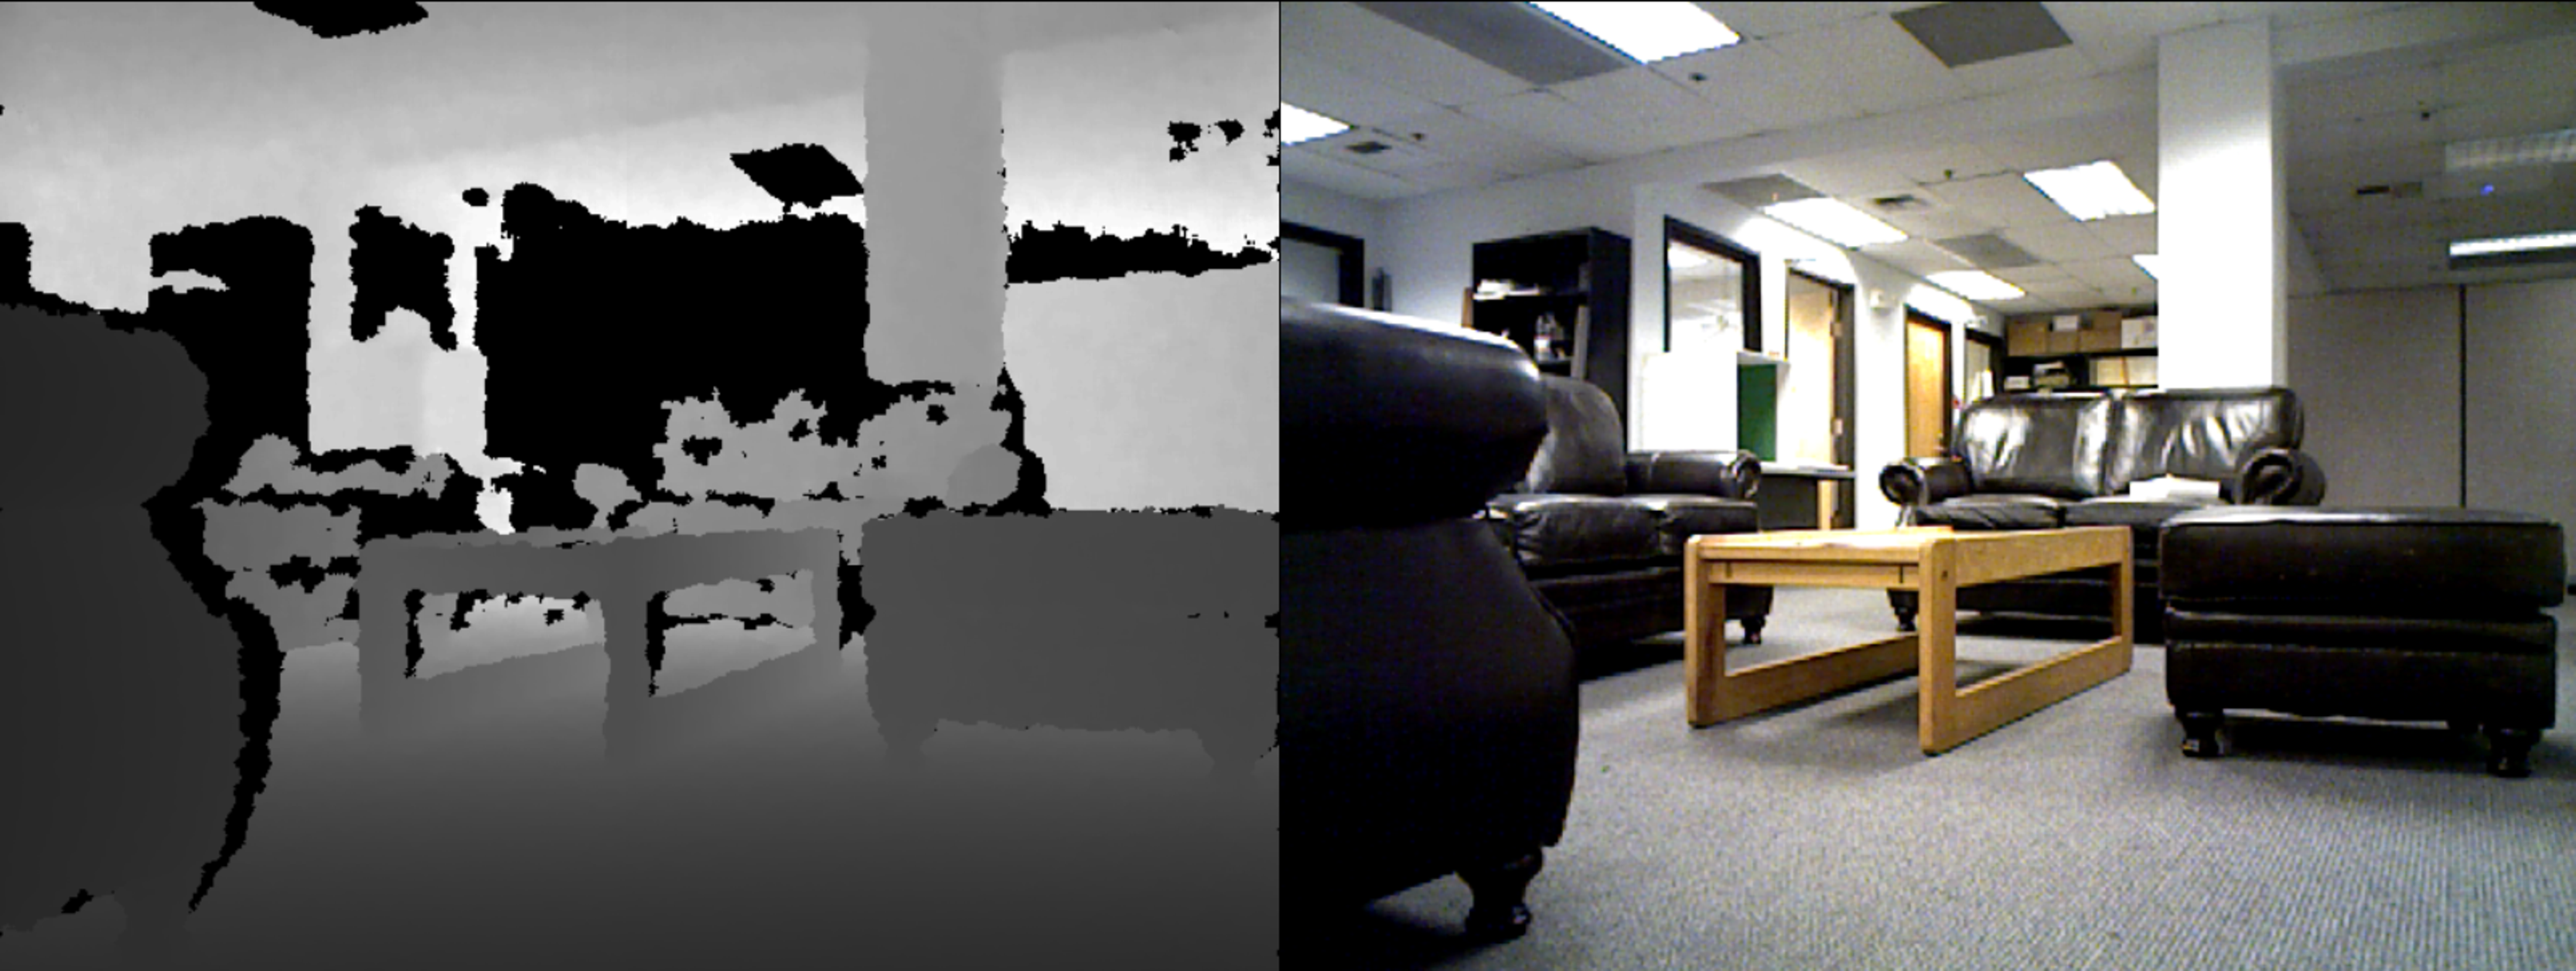
\includegraphics[width=1.0\textwidth]{figures/xtion_rgb_depth}
\caption{\textbf{Sample RGB-D Image Pair}}
\end{figure}
\end{frame}

%----------------------------------------------------------------------------------------

\begin{frame}
\frametitle{Data Flow Block Diagrams}
\begin{figure}
\vspace{-1cm}
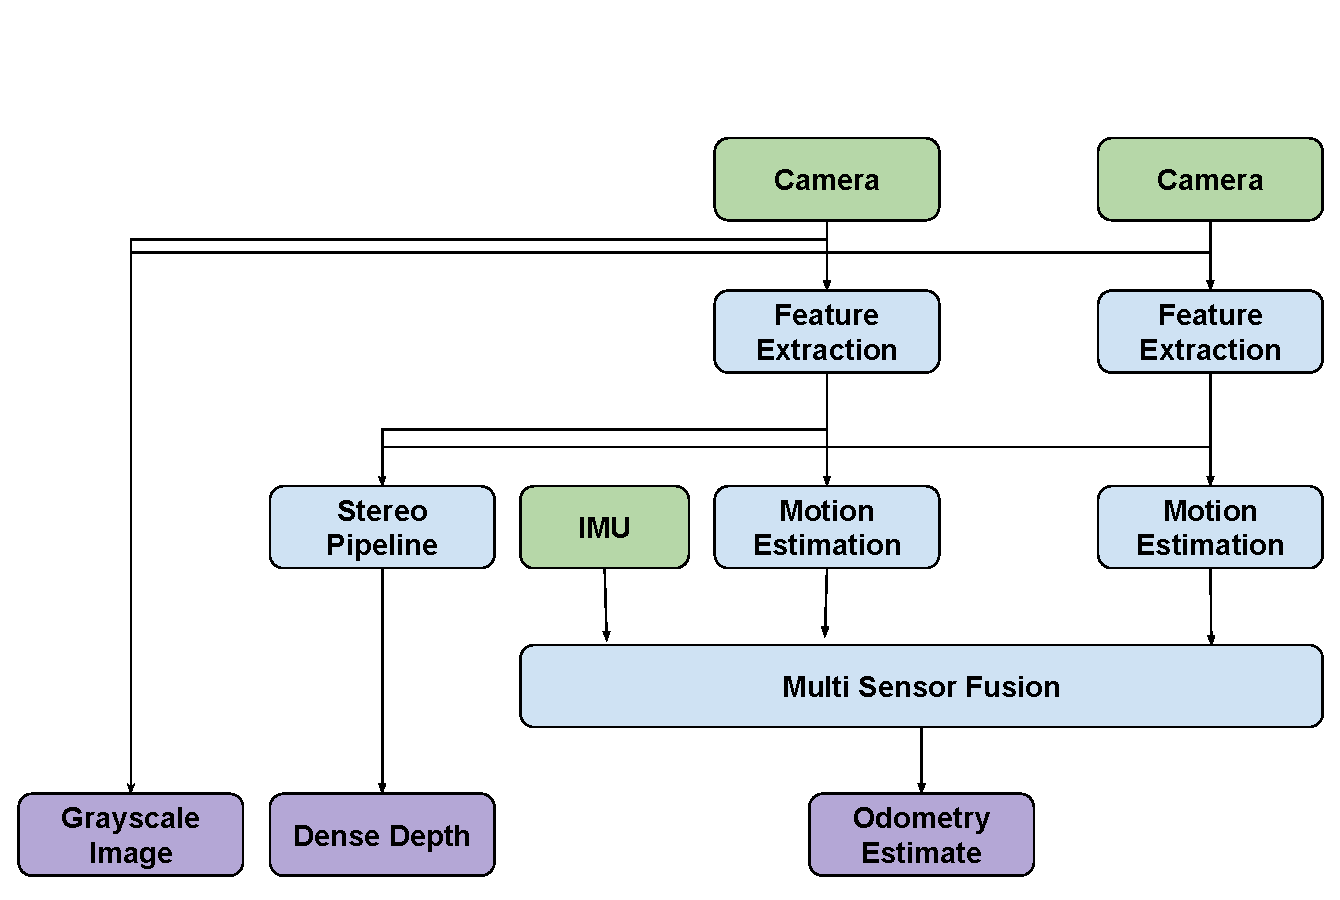
\includegraphics[width=0.9\linewidth]{figures/GuidanceBlock}
\caption{\textit{Guidance} \textbf{ System Diagram}}
\end{figure}
\end{frame}

\begin{frame}
\frametitle{Data Flow Block Diagrams}
\begin{figure}
\vspace{-0.5cm}
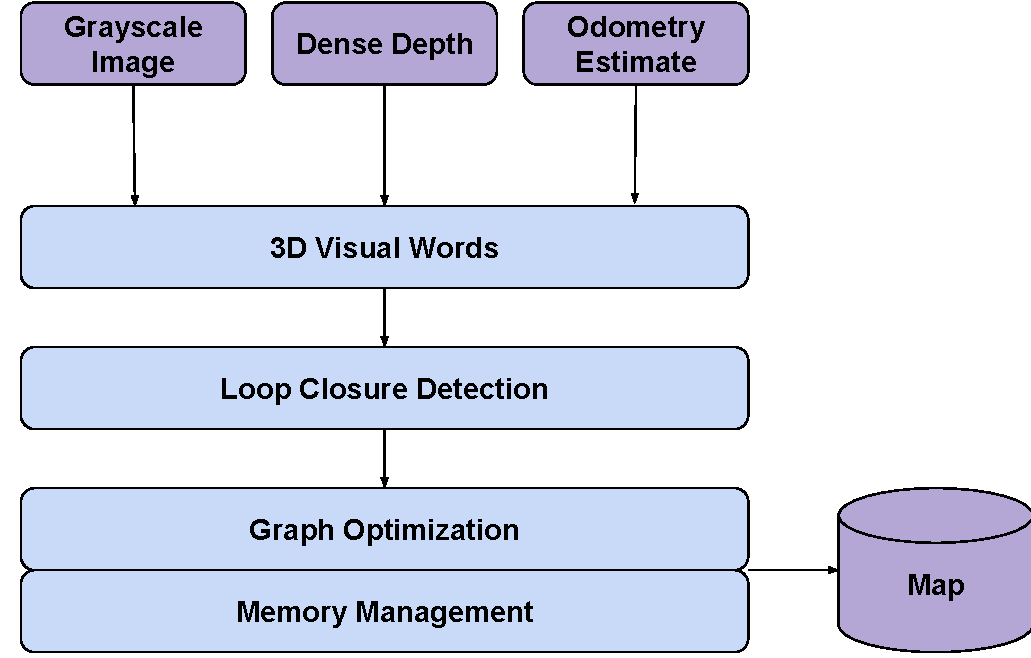
\includegraphics[width=0.8\textwidth]{figures/RTABMapBlock}
\caption{\textit{RTABMap} \textbf{ Mapping System Diagram}}
\end{figure}
\end{frame}

\begin{frame}
\frametitle{\textit{Guidance} Sensor Detail: Camera}
\begin{itemize}
\item{Five stereo pairs, each rectified to pinhole model with available pinhole parameters (10 total cameras)}
\item{QVGA (320x240) resolution in grayscale}
\item{Global shutter}
\item{Auto exposure}
\item{External 20Hz frame rate, synchronized among all cameras}
\end{itemize}
\end{frame}

\begin{frame}
\frametitle{\textit{Guidance} Sensor Detail: IMU}
\begin{itemize}
\item{Five Invensense MPU 6050}
\item{Integrated MEMS gyros + accelerometers}
\item{External 20Hz update rate, synchronized to images}
\end{itemize}
\begin{figure}
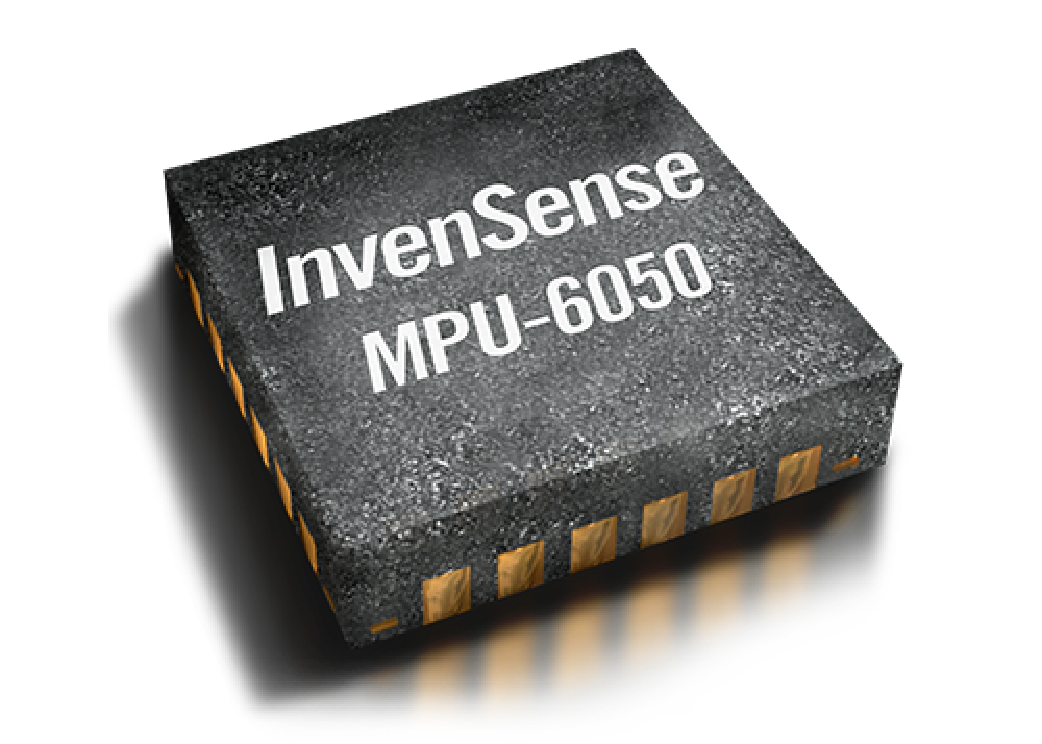
\includegraphics[width=0.3\linewidth]{figures/imu-6050}
\caption{\textit{Invensense} IMU}
\end{figure}
\end{frame}

\section{Processing Algorithms}
\begin{frame}
\frametitle{\textit{Guidance} Processing: Feature Extractor / Descriptor}
\
\begin{itemize}
\item{Independently run on each image (10 total)}
\item{\textbf{FAST}: Features from Accelerated Segment Test}
\item{Relies on corner detection to identify feature}
\item{Characterized by a \textbf{BRIEF} descriptor: Binary Robust Independent Elementary Features}
\item{Optimized for memory-constrained applications}
\end{itemize}

\end{frame}

\begin{frame}
\frametitle{\textit{Guidance} Processing: Motion Estimation}
\begin{itemize}
\item{Uses both 2D$\rightarrow$2D and 3D$\rightarrow$2D estimation}
\item{Monocular estimation based on least squares fit utilizing epipolar constraints and camera calibration parameters}
\item{Stereo estimation utilizes 3D triangulation from stereo calibration parameters}
\item{Seamless switching between mono/stereo motion sources}

\end{itemize}
\end{frame}

\begin{frame}
\frametitle{\textit{Guidance} Processing: Stereo pipeline}
\begin{itemize}
\item{Uses a sliding block matching algorithm}
\item{Computes a dense depth maps for two pairs most aligned in the overall direction of travel}
\item{External 20Hz frame rate of depth map}

\end{itemize}
\end{frame}

\begin{frame}
\frametitle{\textit{Guidance} Processing: Sensor Fusion}
\begin{itemize}
\item{Based on metric scale EKF of Kneip, Weiss, and Siegwart}
\item{Relies on short-term integration of gyro measurements between successive samples}
\item{Incorporates both stereo and mono motion estimates}
\item{External 10Hz data rate}
\end{itemize}
\end{frame}

\begin{frame}
\frametitle{\textit{RTABMap} Processing: 3D Visual Words}
\begin{itemize}
\item{\textbf{SURF} detector: Speeded Up Robust Features}
\item{Faster than \textbf{SIFT}: Scale Invariant Feature Transform}
\item{Not patent encumbered}
\item{Capable of GPU acceleration via OpenCV OpenCL support} 
\item{\textit{Interest points}: Cascaded pyramid using Difference of Gaussians (vs Laplacian of Gaussians for SIFT)}
\item{\textit{Local description}: Based on Haar wavelet response (includes an orientation of the feature for rotation invariance)}
\item{Visual Words combine a SURF feature descriptor with a 3D position}
\end{itemize}
\end{frame}

\begin{frame}
\frametitle{\textit{RTABMap} Processing: Pose Graph Optimization}
\begin{itemize}
\item{SLAM problem represented as a graph: nodes are poses, links are rigid transformations}
\item{Solve by finding minimum residual of estimated poses and estimated transformations that explain measurements}
\item{Optimization only runs using working memory constraints for speed}
\item{Able to run using complete constraints offline for maximum map quality}
\end{itemize}
\begin{figure}
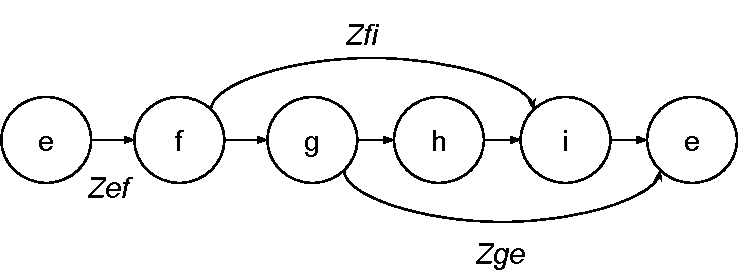
\includegraphics[width=0.5\linewidth]{figures/PoseGraph}
\caption{Pose Graph Representation Showing Rigid Constraints and Loop Closures}
\end{figure}
\end{frame}


\begin{frame}
\frametitle{\textit{RTABMap} Processing: Loop Closure Detection}
\begin{itemize}
\item{Evaluated by comparing extracted visual words of every \textit{N}$^{th}$ frame against saved visual word dictionary}
\item{Creates additional pose graph transformation constraints to limit effect of visual drift}
\item{Rigid transformation estimated using RANSAC over matched visual words}
\end{itemize}
\begin{figure}
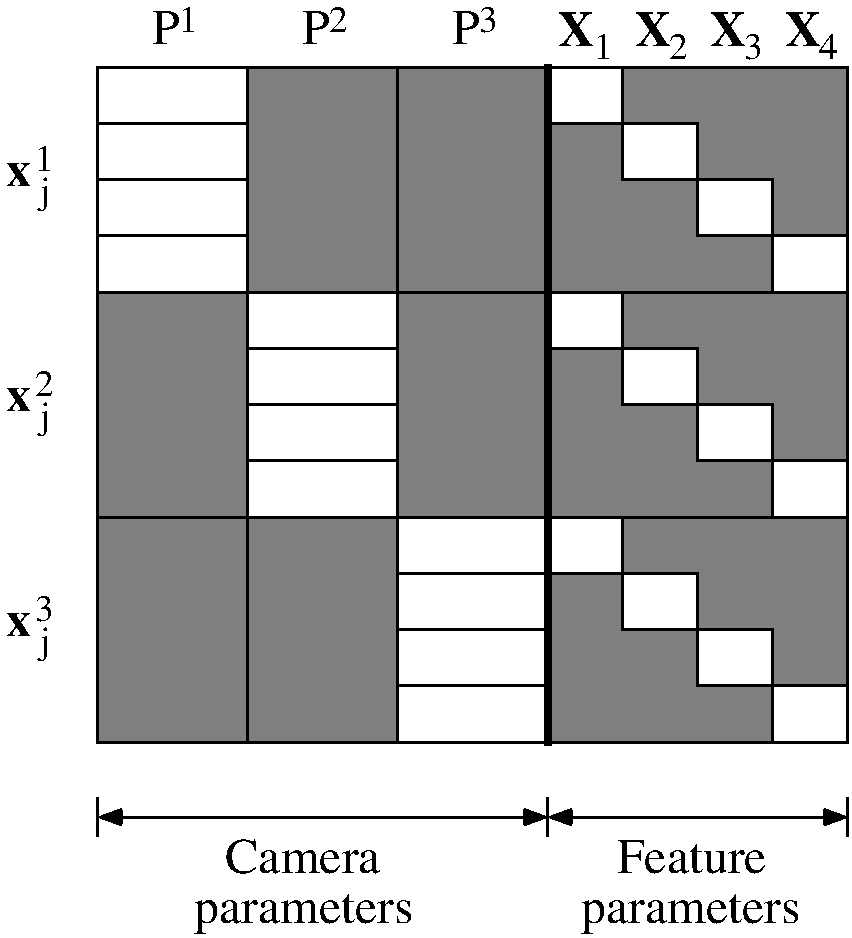
\includegraphics[width=0.3\linewidth]{figures/appendixfigs-sparse-jacobian}
\caption{Pose Graph Sparse Jacobian}
\end{figure}
\end{frame}

\begin{frame}
\frametitle{\textit{RTABMap} Processing: Memory Management}
\begin{itemize}
\item{Three levels of storage of visual words: short-term, working, and long-term}
\item{New data percolate towards long-term memory}
\item{Movement of data is determined by similarity ratio; highly similar images are not stored}
\item{Trades off map quality for online execution of graph optimization over working memory}
\end{itemize}
\end{frame}

\begin{frame}
\frametitle{\textit{RTABMap} Processing: Map Generation}
\begin{itemize}
\item{Map is stored as an OctoMap}
\item{Eight-connected map storing three states: $\{$unknown, empty, known$\}$}
\item{Prepared by projecting depth point clouds from graph optimization into world coordinates}
\end{itemize}
\begin{figure}
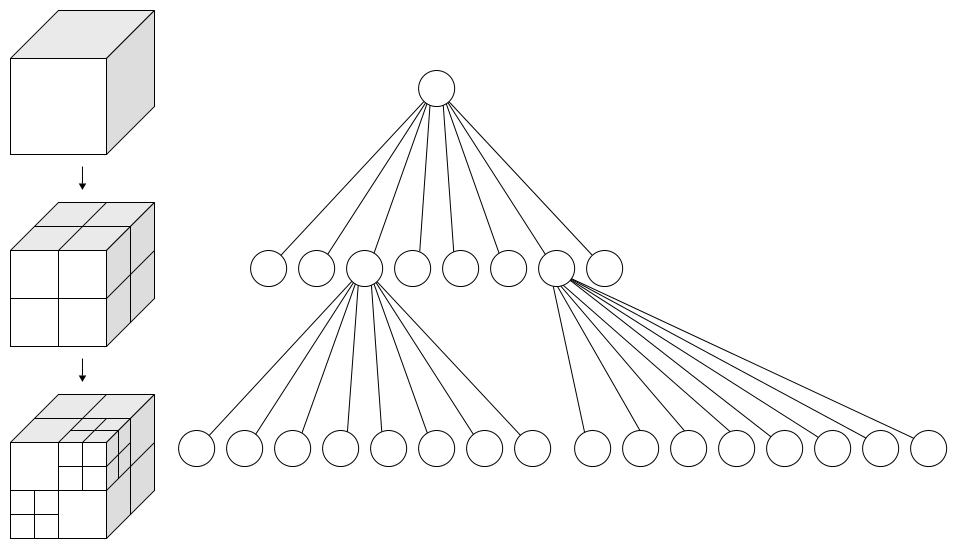
\includegraphics[width=0.6\linewidth]{figures/octree}
\caption{Octree Occupancy Volume Representation}
\end{figure}
\end{frame}


\end{document} 